
%%%%%%%%%%%%%%%%%%%%%%%%%%%%%%%%%%%%%%%%%%%%%%%%%%%%%%%%%%%%%%%%%%%%%%%%%%%%%%%%%%%%%%%
%%%%%%%%%%%%%%%%%%%%%%%%%%%%%%%%%%%%%%%%%%%%%%%%%%%%%%%%%%%%%%%%%%%%%%%%%%%%%%%%%%%%%%%
% 
% This top part of the document is called the 'preamble'.  Modify it with caution!
%
% The real document starts below where it says 'The main document starts here'.

\documentclass[12pt]{article}

\usepackage{amssymb,amsmath,amsthm}
\usepackage[top=1in, bottom=1in, left=1.25in, right=1.25in]{geometry}
\usepackage{fancyhdr}
\usepackage{enumerate}
\usepackage{listings}
\usepackage{graphicx}
\usepackage{float}
\usepackage{multicol}
% Comment the following line to use TeX's default font of Computer Modern.
\usepackage{times,txfonts}
\usepackage{mwe}
\usepackage{caption}
\usepackage{subcaption}

\usepackage{tikz}
\def\checkmark{\tikz\fill[scale=0.4](0,.35) -- (.25,0) -- (1,.7) -- (.25,.15) -- cycle;} 



\makeatletter
\renewcommand*\env@matrix[1][*\c@MaxMatrixCols c]{%
  \hskip -\arraycolsep
  \let\@ifnextchar\new@ifnextchar
  \array{#1}}
\makeatother

\newtheoremstyle{homework}% name of the style to be used
  {18pt}% measure of space to leave above the theorem. E.g.: 3pt
  {12pt}% measure of space to leave below the theorem. E.g.: 3pt
  {}% name of font to use in the body of the theorem
  {}% measure of space to indent
  {\bfseries}% name of head font
  {:}% punctuation between head and body
  {2ex}% space after theorem head; " " = normal interword space
  {}% Manually specify head
\theoremstyle{homework} 

% Set up an Exercise environment and a Solution label.
\newtheorem*{exercisecore}{Exercise \@currentlabel}
\newenvironment{exercise}[1]
{\def\@currentlabel{#1}\exercisecore}
{\endexercisecore}

\newcommand{\localhead}[1]{\par\smallskip\noindent\textbf{#1}\nobreak\\}%
\newcommand\solution{\localhead{Solution:}}

%%%%%%%%%%%%%%%%%%%%%%%%%%%%%%%%%%%%%%%%%%%%%%%%%%%%%%%%%%%%%%%%%%%%%%%%
%
% Stuff for getting the name/document date/title across the header
\makeatletter
\RequirePackage{fancyhdr}
\pagestyle{fancy}
\fancyfoot[C]{\ifnum \value{page} > 1\relax\thepage\fi}
\fancyhead[L]{\ifx\@doclabel\@empty\else\@doclabel\fi}
\fancyhead[C]{\ifx\@docdate\@empty\else\@docdate\fi}
\fancyhead[R]{\ifx\@docauthor\@empty\else\@docauthor\fi}
\headheight 15pt

\def\doclabel#1{\gdef\@doclabel{#1}}
\doclabel{Use {\tt\textbackslash doclabel\{MY LABEL\}}.}
\def\docdate#1{\gdef\@docdate{#1}}
\docdate{Use {\tt\textbackslash docdate\{MY DATE\}}.}
\def\docauthor#1{\gdef\@docauthor{#1}}
\docauthor{Use {\tt\textbackslash docauthor\{MY NAME\}}.}
\makeatother

% Shortcuts for blackboard bold number sets (reals, integers, etc.)
\newcommand{\Reals}{\ensuremath{\mathbb R}}
\newcommand{\Nats}{\ensuremath{\mathbb N}}
\newcommand{\Ints}{\ensuremath{\mathbb Z}}
\newcommand{\Rats}{\ensuremath{\mathbb Q}}
\newcommand{\Cplx}{\ensuremath{\mathbb C}}
%% Some equivalents that some people may prefer.
\let\RR\Reals
\let\NN\Nats
\let\II\Ints
\let\CC\Cplx

%\textbf{Code:}
%\begin{center}
%  \lstinputlisting{NewtonsMethodP5.m}
%\end{center}
%
%\textbf{Console:}
%\begin{center}
%  \lstinputlisting{P5C.txt}
%\end{center}
%\vspace{.15in}


%\begin{figure}[H]
%  \begin{center}
%    \caption{The one-norm unit ball}
%    \includegraphics[width=.76\textwidth]{1norm.png}
%  \end{center}
%\end{figure}




%%%%%%%%%%%%%%%%%%%%%%%%%%%%%%%%%%%%%%%%%%%%%%%%%%%%%%%%%%%%%%%%%%%%%%%%%%%%%%%%%%%%%%%
%%%%%%%%%%%%%%%%%%%%%%%%%%%%%%%%%%%%%%%%%%%%%%%%%%%%%%%%%%%%%%%%%%%%%%%%%%%%%%%%%%%%%%%
% 
% The main document start here.

% The following commands set up the material that appears in the header.
\doclabel{Math 661: Homework 1}
\docauthor{Stefano Fochesatto}
\docdate{\today}


\begin{document}


\begin{exercise}{2.1} Consider the feasible region defined by the constrains, 
  \begin{equation*}
    1 - x_1^2 - x_2^2 \geq 0, \sqrt{2} - x_1 - x_2 \geq 0,\text{ and } x_2 \geq 0. 
  \end{equation*}
  For each of the following points, determine whether the point is feasible or infeasible and (if it is feasible)
  whether it is interior to or on the boundary of each of the constraints:
  \begin{enumerate}
    \item $x_a = (\frac{1}{2}, \frac{1}{2})^{T}$.
    \solution Checking constraints, 
    \begin{equation*}
      1 - \left(\frac{1}{2}\right)^2 - \left(\frac{1}{2}\right)^2 = 1 - \frac{2}{4} = \frac{1}{2} > 0
    \end{equation*}
    \begin{equation*}
      \sqrt{2} - (\frac{1}{2}) - (\frac{1}{2}) = \sqrt{2} - 1 > 0
    \end{equation*}
    and clearly $\frac{1}{2} > 0$. Thus $x_a$ is a feasible point, and since we have strict inequalities
    on all the constraints we know that $x_a$ is interior to all constraints (Defined in Chapter 2 p.44). 
    
    \item $x_b = (1,0)^T$
    \solution Checking all constraints, 
    \begin{equation*}
      1 - 1^2 - 0^2 = 1 - 1 =  0
    \end{equation*}
    \begin{equation*}
      \sqrt{2} - (1) - (0) = \sqrt{2} - 1 > 0
    \end{equation*}
    and since $x_2 = 0$ we know that $x_b$ is a feasible point. Note that $x_b$ is on the boundary of 
    $1 - x_1^2 - x_2^2 \geq 0$ and $x_2 \geq 0$, and interior to $\sqrt{2} - x_1 - x_2 \geq 0$.


    \item $x_c = (-1, 0)^T$
    \solution Checking all constraints, 
    \begin{equation*}
      1 - (-1)^2 - 0^2 = 1 - 1 =  0
    \end{equation*}
    \begin{equation*}
      \sqrt{2} - (-1) - (0) = \sqrt{2} + 1 > 0
    \end{equation*}
    and since $x_2 = 0$ we know that $x_c$ is a feasible point. Note that $x_c$ is on the boundary of 
    $1 - x_1^2 - x_2^2 \geq 0$ and $x_2 \geq 0$, and interior to $\sqrt{2} - x_1 - x_2 \geq 0$.

    \item $x_d = (-\frac{1}{2}, 0)^T$ 
    \solution Checking all constraints, 
    \begin{equation*}
      1 - (-\frac{1}{2})^2 - 0^2 = 1 - \frac{1}{4} =  \frac{3}{4} > 0
    \end{equation*}
    \begin{equation*}
      \sqrt{2} - (-\frac{1}{2}) - (0) = \sqrt{2} + \frac{1}{4} > 0
     \end{equation*}
     and since $x_2 = 0$ we know that $x_d$ is a feasible point. Note that $x_d$ is on the boundary of $x_2 \geq 0$, and 
     interior to $1 - x_1^2 - x_2^2 \geq 0$ and  $\sqrt{2} - x_1 - x_2 \geq 0$.

    \item $x_e = (1/\sqrt{2}, 1/\sqrt{2})^T$?
    \solution 
    Checking all constraints, 
    \begin{equation*}
      1 - (\frac{1}{\sqrt{2}})^2 - (\frac{1}{\sqrt{2}})^2 = 1 - \frac{1}{2} - \frac{1}{2} = 0 
    \end{equation*}
    \begin{equation*}
      \sqrt{2} - (\frac{1}{\sqrt{2}}) - (\frac{1}{\sqrt{2}}) = 0
    \end{equation*}
    and since $1/\sqrt{2} > 0$ we know that $x_e$ is a feasible point. Note that $x_d$ is on the boundary of $1 - x_1^2 - x_2^2 \geq 0$ and  $\sqrt{2} - x_1 - x_2 \geq 0$,
    and is interior to $x_2 \geq 0$.
  \end{enumerate}
\end{exercise}
\vspace{1in}

%%% Add image
\begin{exercise}{2.3} Consider the problem, 
  \begin{align*}
    \text{minimize } f(x) &= x_1,\\
    \text{subject to } x_1^2 + x_2^2 &\leq 4\\
    x_1^2 &\geq 1.
  \end{align*}
  Graph the feasible set. Use the graph to find all local minimizers for the problem, and determine which of those are also global minimizers.
  \solution Consider the following plot of the feasible set. 
  \begin{figure}[H]
    \begin{center}
      \caption{Feasible set $S$ denoted in green.}
      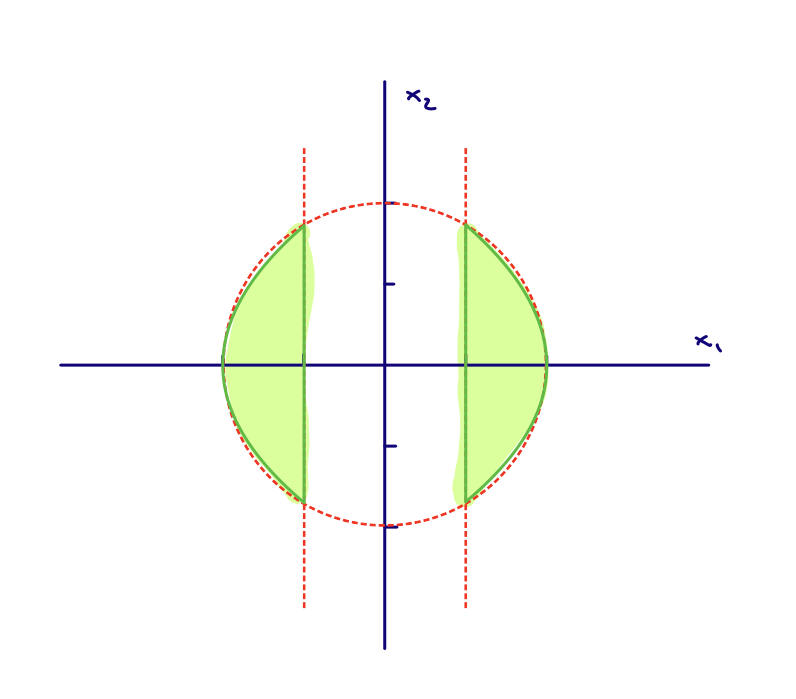
\includegraphics[width=.76\textwidth]{Example1.png}
    \end{center}
  \end{figure}

  Since the objective function is $f(x) = x_1$ it's clear that there are a set of local minimizers when $x_1 = 1$, and $x_2 \leq \pm\sqrt{3}$.
  There is a single global minimizer where $x_1 = -2$, and $x_2 = 0$.  
\end{exercise}
\vspace{1in}




%%% Add image
\begin{exercise}{2.4}Consider the problem, 
  \begin{align*}
    \text{minimize } f(x) &= x_1,\\
    \text{subject to } (x_1 - 1)^2 + x_2^2 & = 1\\
    (x_1 + 1)^2 + x_2^2 & = 1.
  \end{align*}
  Graph the feasible set. Use the graph to find all local minimizers for the problem, and determine which of those are also global minimizers.
  \solution Consider the following plot of the feasible set. 
  \begin{figure}[H]
    \begin{center}
      \caption{Feasible set $S$ denoted in green.}
      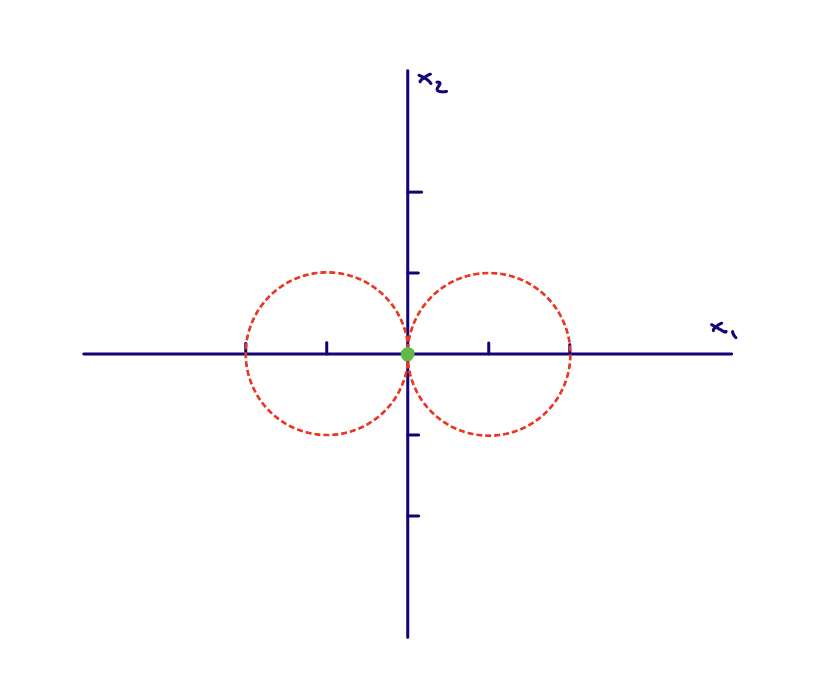
\includegraphics[width=.76\textwidth]{example2.png}
    \end{center}
  \end{figure}

  Since the feasible set contains only one point, namely $x_1 = 0$, $x_2 = 0$ it must be the global minimizer. 
\end{exercise}
\vspace{1in}


%%% Add image
\begin{exercise}{2.5} Give an example of a function that has no global minimizer and no global maximizer.\\
  \solution Consider the function $f(x) = 1/x$ on the interval $[-2, 2]$. 
  \begin{figure}[H]
    \begin{center}
      \caption{Objective function on feasible set $x \in [-2,2]$.}
      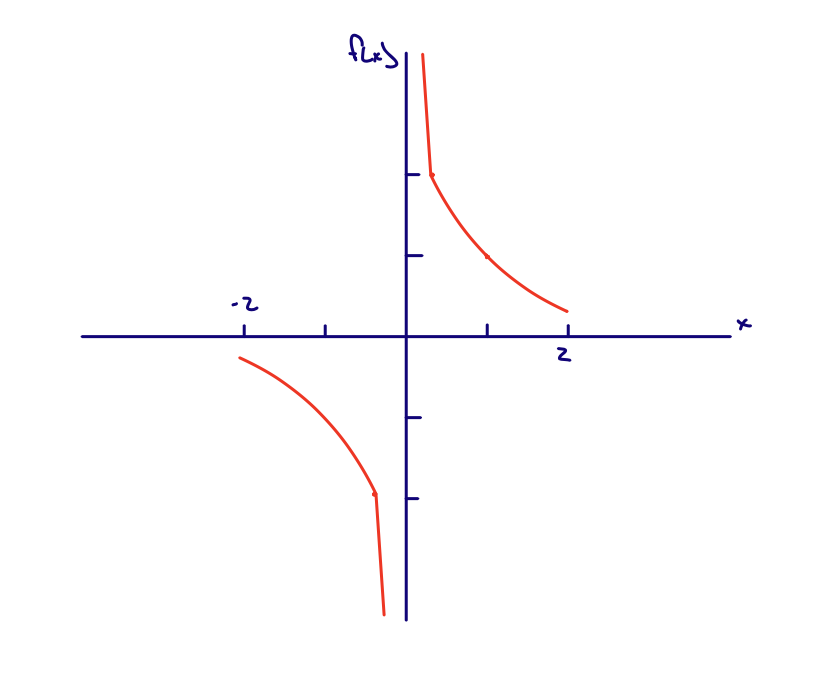
\includegraphics[width=.76\textwidth]{example3.png}
    \end{center}
  \end{figure}
  Note that there is a local minimizer at $x = 2$ but clearly any global minimizer will be on the interval $[-2, 0)$. Since 
  $f(x)$ is strictly decreasing and divergent as $x$ approaches 0, it is impossible to construct an $\epsilon$-neighborhood around any $x_*$ such that
  $f(x_*) \leq f(x)$ for all $x \in [-2, 0)$.\\
  
  Similarly any global maximizer must be on the interval $(0, 2]$. Since $f(x)$ is strictly decreasing and divergent as $x$ approaches $0$, it is also impossible to 
  construct an $\epsilon$-neighborhood around any $x_*$ such that
  $f(x_*) \geq f(x)$ for all $x \in (0, 2]$.
\end{exercise}
\vspace{1in}



\begin{exercise}{Problem P1} Solve calcone by implementing a strategy for solving this and similar one-variable optimization problems on bounded, closed intervals. 
  Describe the strategy in brief and well-written english. Your strategy will necessarily be iterative, and will not get the exact answer but only an approximate one.
  Discuss any issues about the general performance/success of your strategy, emphasizing how it might fail on problems of this type. Argue that you answer to this particular problem is given 
  to at least 6-digit accuracy, and along the way visualize the function $f(x)$.\\
  \begin{align*}
    \text{minimize } f(x) &= (x^2 + \sin(x))^2 - 10\left(\cos(5x) + \frac{3}{2}x\right),\\
    \text{on the interval } S & = [0,2]
  \end{align*}
  \solution The strategy I implemented for solving this problem is the minimization analog to bisection root finding. Consider a function $f$ on a closed interval $[a, b]$. Consider points $u, v \in [a, b]$ such that 
  $u < v$. Compute $f(u)$ and $f(v)$. If $f(u) > f(v)$ then there must exist a local minimum on the set $[u,b]$. Similarly if $f(v)>f(u)$ there must exist a local minimum on the set $[a,v]$. We repeat this iteratively until the interval becomes essentially 
  an $\epsilon$ neighborhood of a local minimum. Clearly a function could exploit this method, consider the following plot if we were to let $u = .4$ and $v = .5$ the method would converge to the local minimum near 0. 
  \begin{figure}[H]
    \begin{center}
      \caption{Bisection Counter Example}
      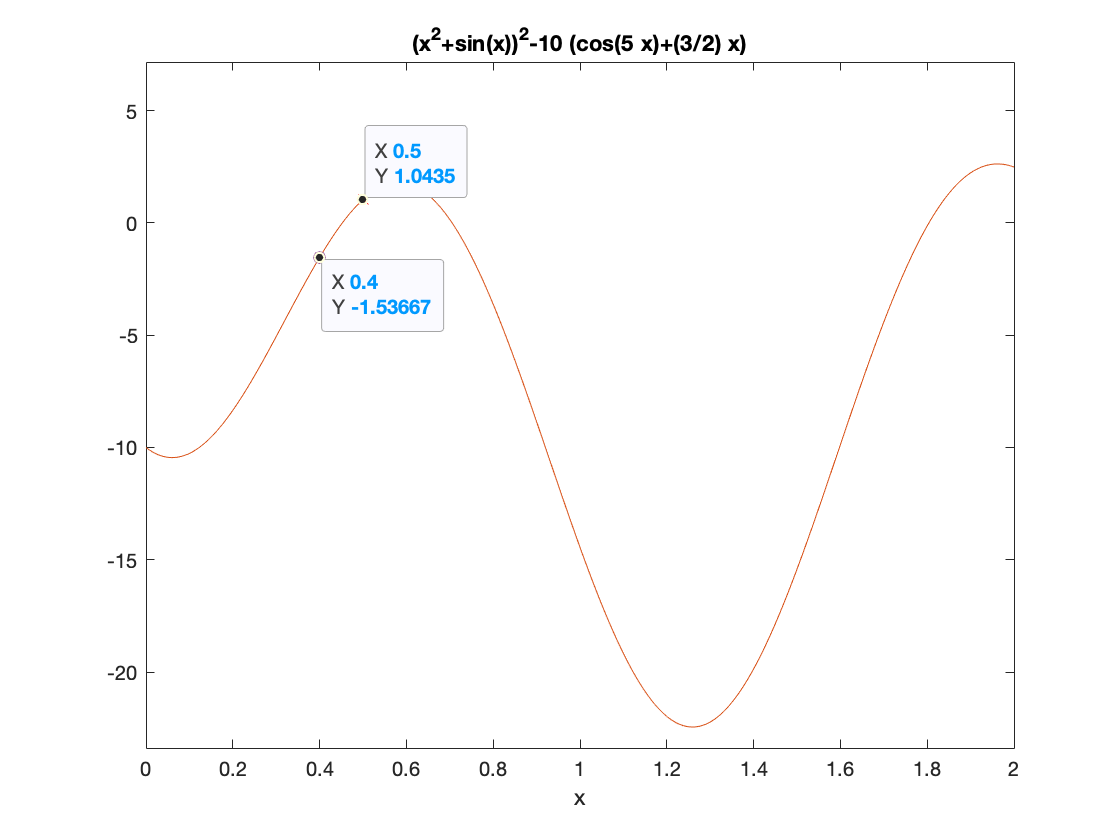
\includegraphics[width=.76\textwidth]{calcone.png}
    \end{center}
  \end{figure}

  To counter this I propose we take several equally spaced intervals on $[a,b]$ small enough such that the function on any sub-interval $[x_i, x_{i +1}]$ contains very little change in concavity. The final code (looks like psuedocode;)\\

  \textbf{Code:}
  \begin{center}
    \lstinputlisting[basicstyle = \footnotesize]{r1.txt}
  \end{center}
  \textbf{Console:}
  \begin{center}
    \lstinputlisting[basicstyle = \footnotesize]{r2.txt}
  \end{center}
  \vspace{.15in}

  We exit the recursion when the bounds of the current interval, say $[a, b]$ are smaller than $10^{-6}$. Since we know the interval $[a,b]$ must contain a local minimum
  any point within $[a,b]$ will also be within 6 digits accuracy to the true minimum in $[a, b]$.
  \vspace{1in}

  \begin{exercise}{Problem P2} Solve fit. Follow essentially the same rules as the previous problem. Describe a strategy for solving 
    this and similar problems. Discuss any issues about the general performance/ success of your strategy. Implement your strategy as Matlab code.
    Demonstrate 6 digits of accuracy. Plot the solution curve on the same graph as the data.\\
    \solution Note that we are aiming to fit $\hat{c}$ of the function 
    \begin{equation*}
      g(x) = c_1 + c_2x + c_3e^{-5x},
    \end{equation*}
    Such that the sum of squares to our data points are minimized. Therefore for every $y_i$ we seek to minimize $e_i$ and generally the sum squared error $\frac{1}{2}\sum \epsilon_i^2$, 
    \begin{equation*}
      y_i = c_1 + c_2x_i + c_3 + \epsilon_i.
    \end{equation*}
    Consider the following system of equations, 
    \begin{align*}
      \begin{bmatrix}
        y_1\\
        y_2\\
        \vdots \\
        y_{11}
      \end{bmatrix}
       &=
       \begin{bmatrix}
        1 && x_1 && e^{-5x_1}\\
        1 && x_2 && e^{-5x_2}\\ 
        \vdots && \vdots && \vdots\\ 
        1 && x_{11} && e^{-5x_{11}}
       \end{bmatrix}
       \begin{bmatrix}
        c_1\\
        c_2\\
        c_3
       \end{bmatrix}
        + 
        \begin{bmatrix}
          \epsilon_1\\
          \epsilon_2\\
          \vdots \\
          \epsilon_{11}
        \end{bmatrix}\\
        \hat{y} &= X\hat{c} + \hat{\epsilon}.
    \end{align*}    
    Solving for $\hat{\epsilon}$ we get, 
    \begin{equation*}
      \hat{\epsilon} = \hat{y} - X\hat{c}.
    \end{equation*}
    Applying sum of square over two we get, what is essentially the given objective function. 
    \begin{equation*}
      f(\hat{c}) = \frac{1}{2}\hat{\epsilon}'\hat{\epsilon} = \frac{1}{2}(\hat{y}' - \hat{c}'X')(\hat{y} - X\hat{c}).
    \end{equation*}
    Expanding the right hand side. 
    \begin{equation*}
      f(\hat{c}) =  \frac{1}{2}(\hat{y}'\hat{y} - \hat{y}'X\hat{c}  - \hat{c}'X'\hat{y} + \hat{c}'X'X\hat{c}) = \frac{1}{2}(\hat{y}'\hat{y} - 2\hat{c}'X'\hat{y} + \hat{c}'X'X\hat{c})
    \end{equation*}
    Taking the gradient of our objective function in terms of $\hat{c}$,
    \begin{equation*}
      f'(\hat{c}) = \frac{1}{2}(-2X'y + 2X'X\hat{c}) = -X'y + X'X\hat{c}
    \end{equation*}
    Setting our gradient, $f'(\hat{c}) = \hat{0}$ and and solving for $\hat{c}$ we get the following system of equations, 
    \begin{align*}
    -X'y + X'X\hat{c} &= 0,\\
    X'X\hat{c} &= X'y,\\
    \hat{c} &= (X'X)^{-1}X'y.
    \end{align*}
    Our procedure for solving this problem will continue by using in-place householder decomposition on $X'X$, forming $Q^*X'y$, and then solving for 
    $\hat{c}$ via back substitution. \\

    \textbf{Code:}
    \begin{center}
      \lstinputlisting[basicstyle = \footnotesize]{r3.txt}
    \end{center}
    \textbf{Console:}
    \begin{center}
      \lstinputlisting[basicstyle = \footnotesize]{r4.txt}
    \end{center}
    \vspace{.15in}

    \begin{figure}[H]
      \begin{center}
        \caption{Plot of $f(x) = 1.82 - 2.75x + 3.15e^{-5x}$}
        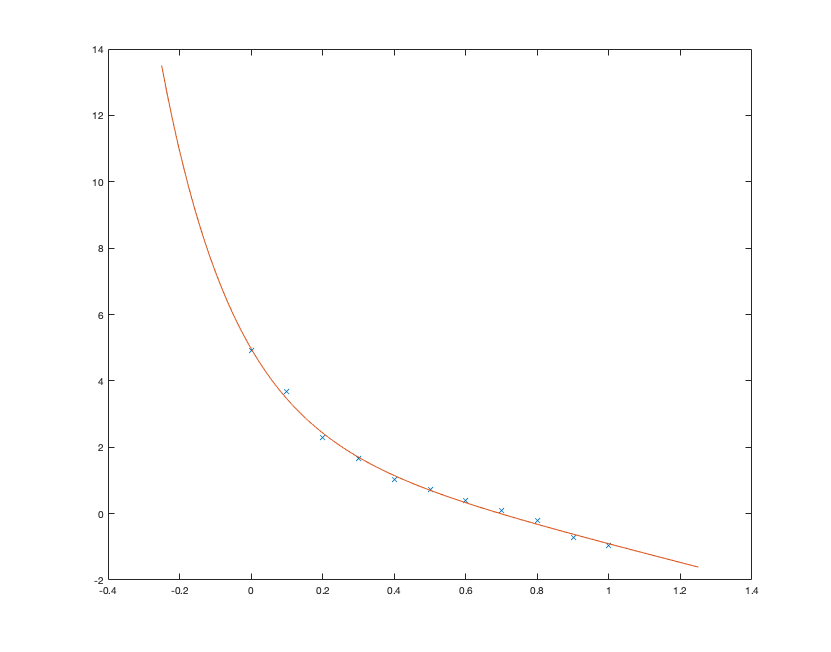
\includegraphics[width=.76\textwidth]{fit.png}
      \end{center}
    \end{figure}
    The flops for solving a triangular system is $O(n^2)$ and Householder decomposition is $O(n^3)$, so this method finds the optimal 
    $\hat{c}$ in $O(n^3)$. (Reference NLA Trefethen, Bau Algorithm 11.2 p.83)
  \end{exercise}

  \vspace{.15in}


  \begin{exercise}{Problem P3} Solve Salmon. In fact this problem is embarrassingly simple to solve. Start by writing a few clear sentences 
    stating and justifying the solution. Then visualize, in 3D and probably with pencil and paper, the set of feasible solutions; mark and label the solution on this plot. 
    Also use a straightforward substitution to eliminate the equality constraint, and then re-visualize the feasible set and solution in 2D. Is this problem discrete? Is it fait to interpret it as 
    continuous? Comment. \\

    Salmon is a constrained minimization problem where the goal is to minimize, 
    \begin{equation*}
      f(x) = 2x_1 + 3x_2 + 4x_3
    \end{equation*}
    subject to. 
    \begin{align*}
      x_1 + x_2 &+ x_3 = 22\\
      0 \leq &x_1 \leq 2\\
      0 &\leq x_2\\
      4 \leq &x_3 \leq 10.
    \end{align*}
    \solution Note that the total number of fish is 22 as denoted by the first constraint. Since $x_1$ contributes the least to increasing $f(x)$ it follows that we should maximize $x_1$ under the $0 \leq 0 \leq 2$ constraint. 
    Therefore $x_1 = 2$, and thus we have that $x_2 + x_3 = 20$. Since $x_3$ contributes the most to increasing $f(x)$ it also follows that we should minimize $x_3$ under the $4 \leq x_3 \leq 10$ constraint. Thus $x_3 = 4$ and
    we $x_2 = 16$. Shifting the values to lower $x_1$ or raise $x_3$ results in a larger $f(x)$ and thus $x = [2, 16, 4]'$ minimizes $f(x)$. Consider the following plot of the feasible set, 
    \begin{figure}[H]
      \begin{center}
        \caption{Feasible set $S$ denoted in green.}
        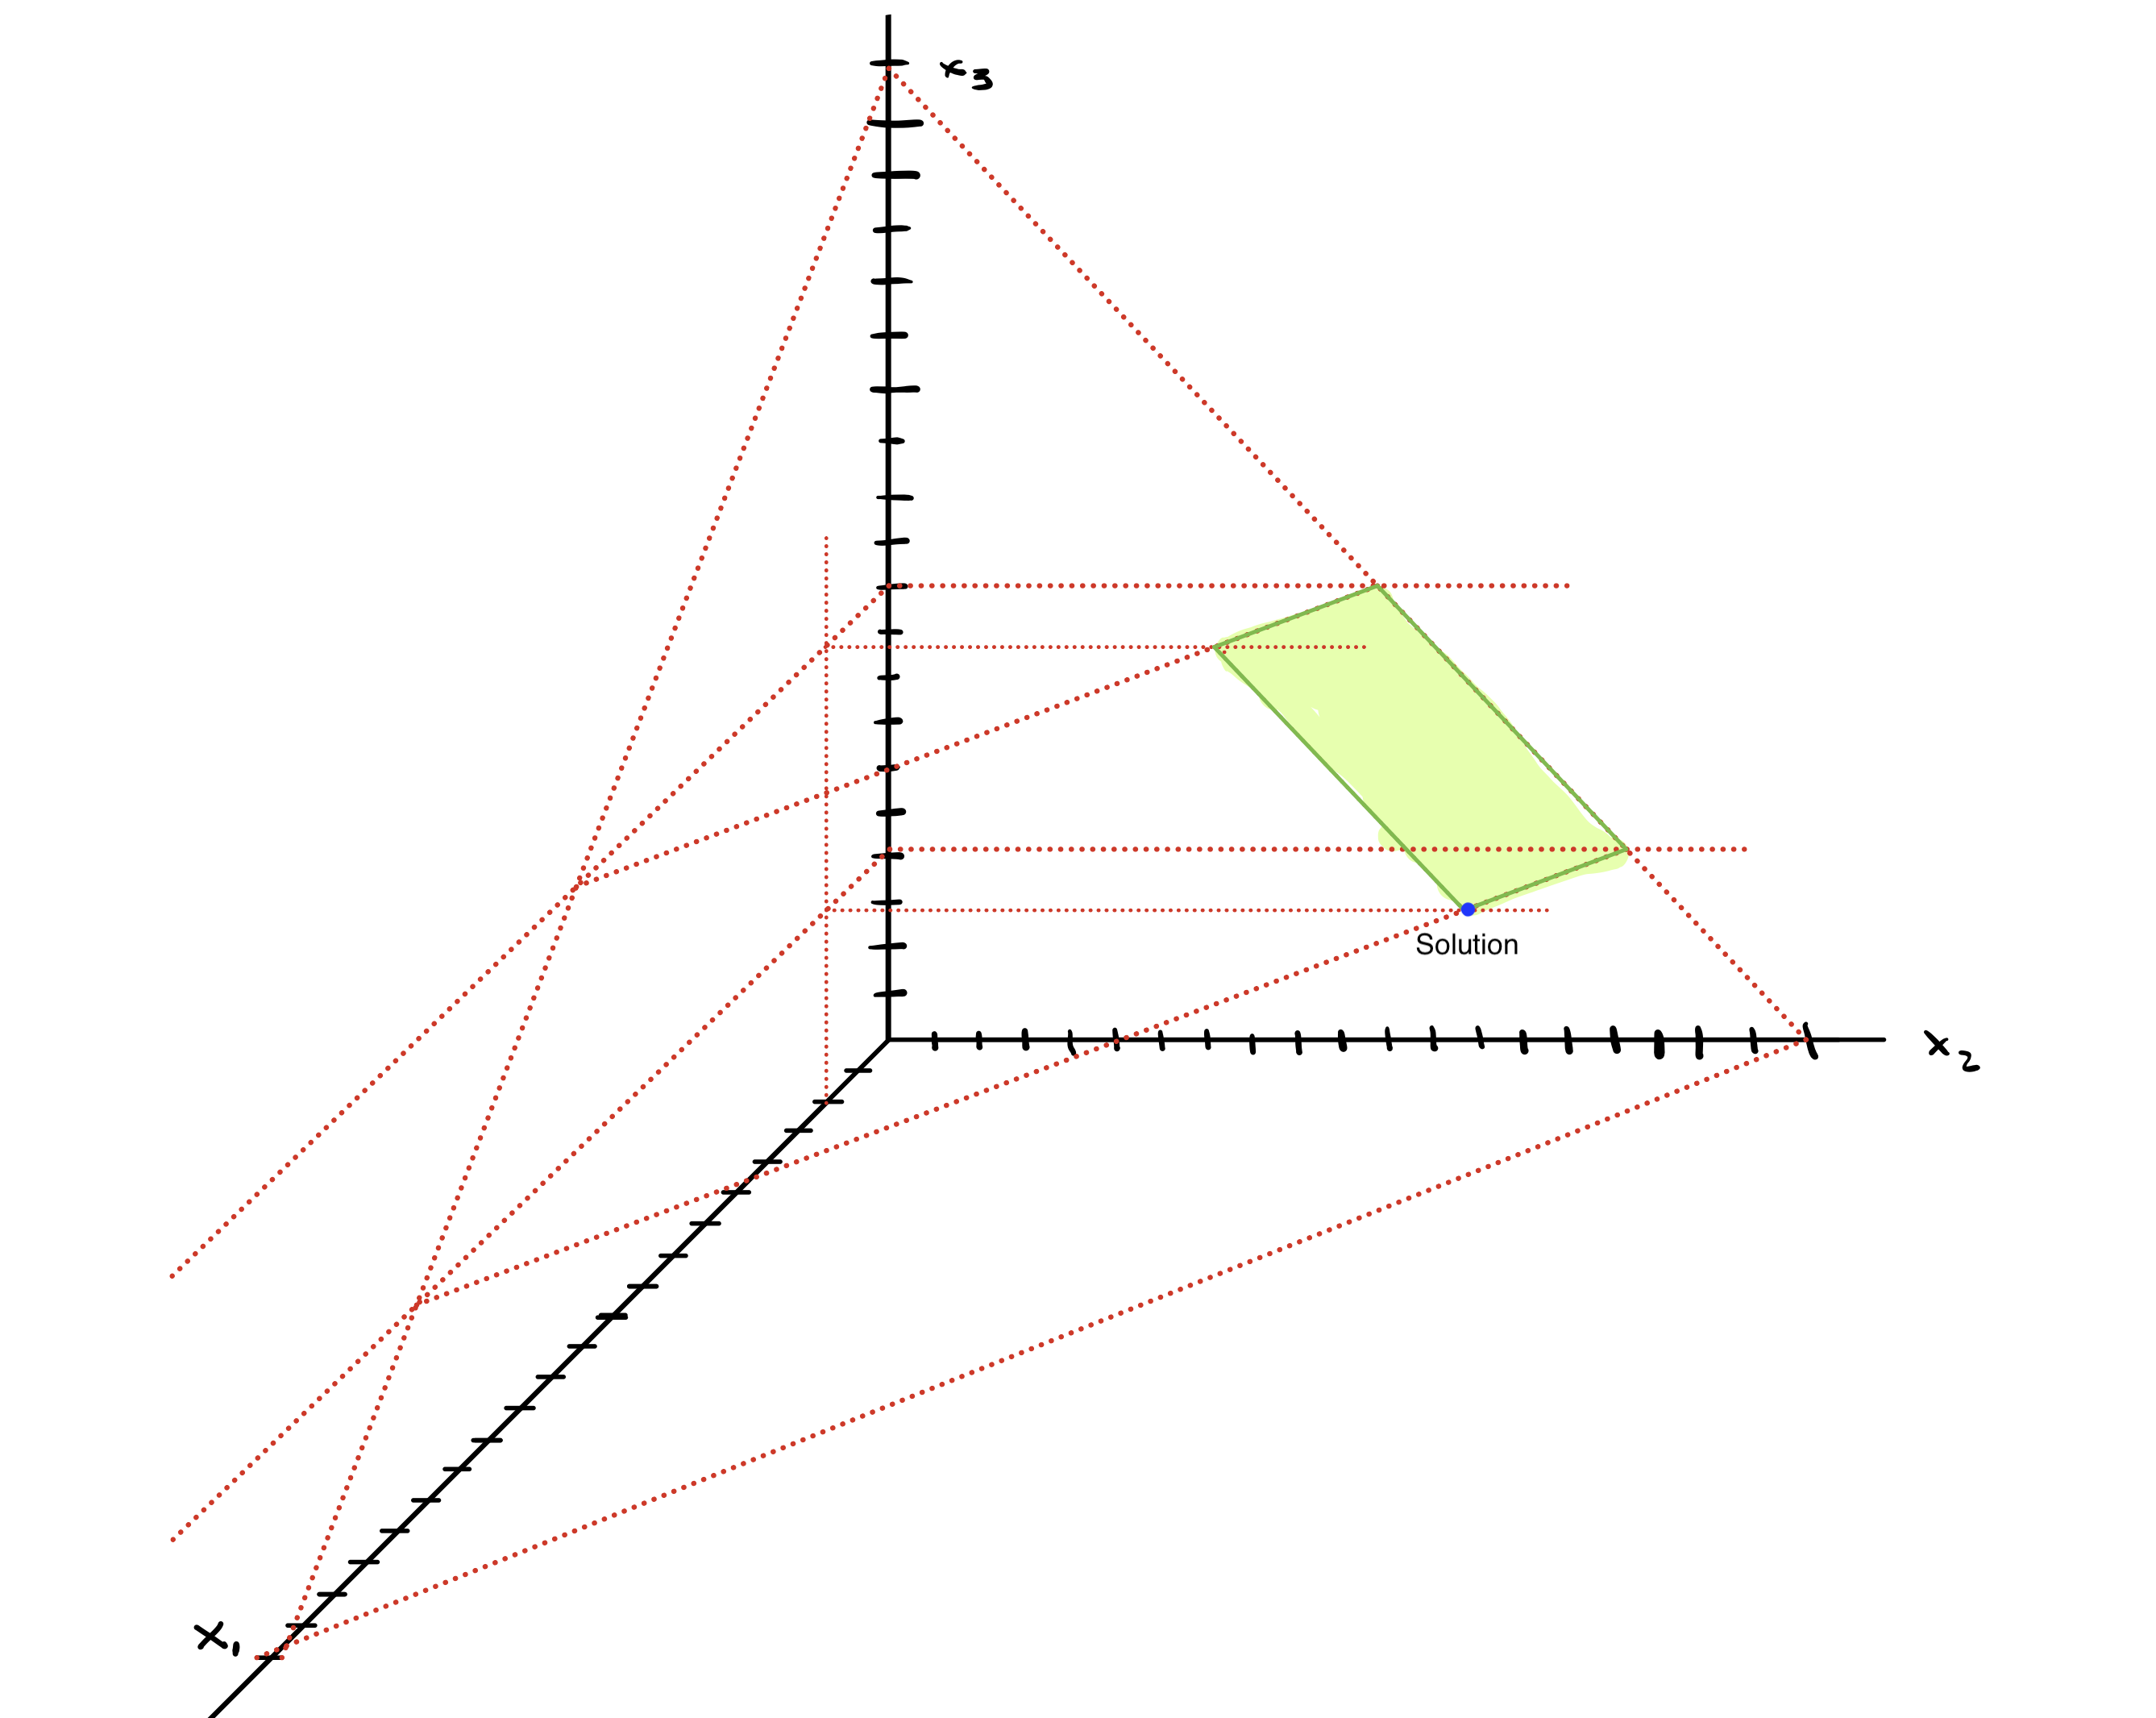
\includegraphics[width=.76\textwidth]{FeasibleSet.png}
      \end{center}
    \end{figure}
    Solving the equality constraint for $x_3$ we get the following problem, 
    \begin{equation*}
      f(x) = 2x_1 + 3x_2 + 4(22 - x_1 - x_2) = -2x_1-x_2+88
    \end{equation*}
    subject to. 
    \begin{align*}
      0 \leq &x_1 \leq 2,\\
      0 &\leq x_2,\\
      18 \geq &x_1 + x_2\geq 12.
    \end{align*}
    Now the feasible set can be visualized in two dimensions, 
    \begin{figure}[H]
      \begin{center}
        \caption{Two dimensional feasible set $S$ denoted in green.}
        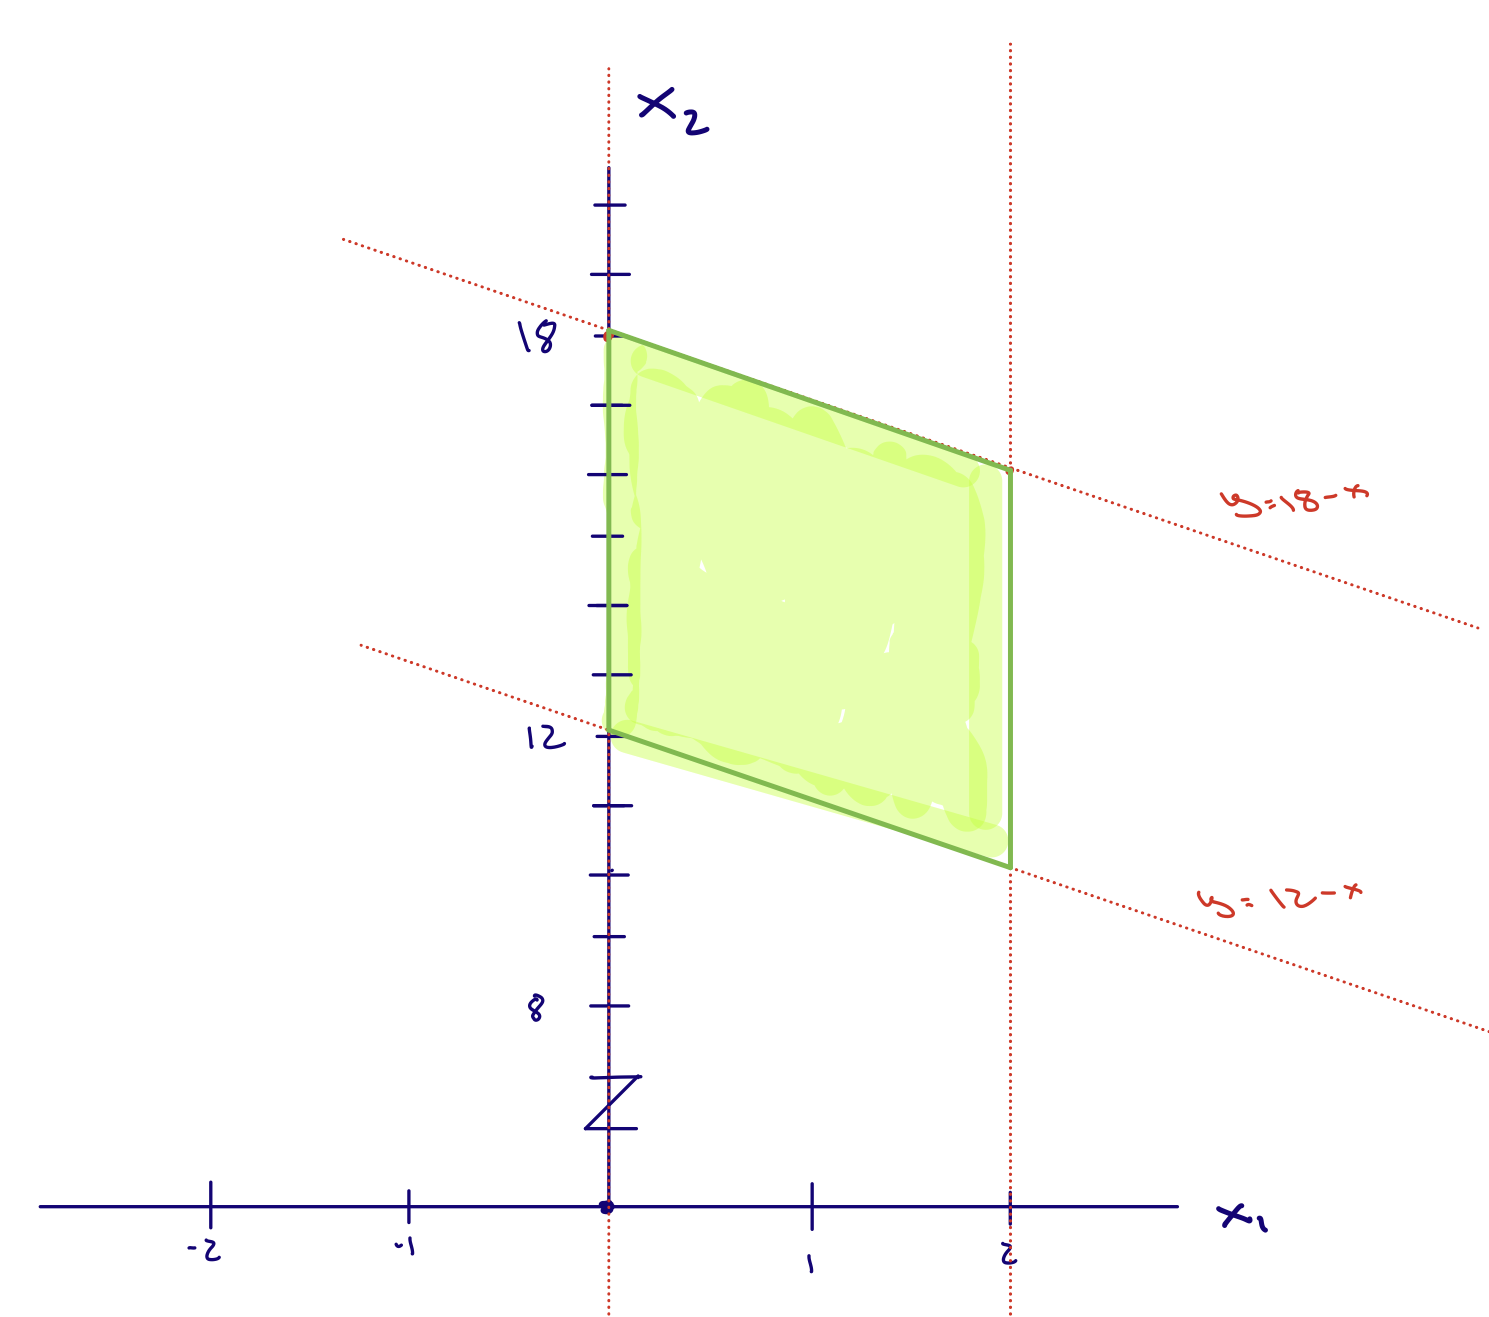
\includegraphics[width=.76\textwidth]{2dsalmon.png}
      \end{center}
    \end{figure}
    Given the context of the problem, we are looking for some discrete answer, whether it's in a multiple of $1/8$ or 1 whole of a salmon. However we treat the problem as continuous i.e. our feasible set is continuous.
  \end{exercise}
  \vspace{.15in}



  \begin{exercise}{Problem P4} Complete the following classification table for the example problems:
    \solution 
    \begin{center}
      \begin{tabular}{c | c | c | c | c | c |} 
        name & discrete & constrained & linear & quadratic & dimension\\ 
        \hline
        calcone &  &   &  &  \checkmark & 1\\
        \hline
        fit &  &  & \checkmark &  \checkmark & 3\\
        \hline
        salmon & \checkmark (in interpretation) & \checkmark & \checkmark & \checkmark & 3\\
        \hline
        tsp & \checkmark & \checkmark &  &  & n \\
        \hline
        glacier &  & \checkmark &  &  & $\infty$ \\
        \hline
      \end{tabular}
      \end{center}
    
  \end{exercise}











  
\end{exercise}









\end{document}


































